\section{Abbreviated Related Work}
\label{sec:related_work}


\textbf{Conservative model-based optimization:}
A standard approach to safe policy improvement relies on the observation that the risk of a new policy can be bounded in terms of the risk of a reference policy plus a penalty that grows with the divergence between them \citep{kakade2002approximately}.
When the reference policy is known to satisfy the safety constraint, controlling this divergence provides a mechanism for controlling risk.
The idea of bounding risk through bounded divergence motivates a broad family of locality-constrained policy optimization methods \citep{kim2025offline}.
Prior work has proposed entropy-regularized control and KL-penalized objectives \citep{todorov2009efficient, fox2015taming}, trust-region policy optimization \citep{schulman2015trust, schulman2017proximal}, conservative value penalties in offline reinforcement learning \citep{kumar2020conservative, trabucco2021conservative}, trust-region methods in black-box optimization \citep{eriksson2019scalable}, and uncertainty-penalized safe Bayesian optimization \citep{sui2015safe}.
\citet{damani2023beyond} proposed using a likelihood ratio as a safety filter for model-based optimization, but treated the ratio threshold as a hyperparameter.

From an optimization perspective, our work is most similar to \citet{stanton2023bayesian}, who proposed constraining a Bayesian optimization policy to regions where the resulting conformal prediction sets would have bounded width given a declared miscoverage tolerance $\alpha$.
However, their approach was limited by three weaknesses.
First, their approach was restricted to the miscoverage loss.
Second, their use of an implicit policy created an awkward fixed-point problem: finding the policy that induced an action distribution that controlled the coverage.
%under which the coverage would be controlled.
Third, they did not fully address the multi-step feedback covariate shift induced by sequential model-based optimization.\footnote{A form of covariate shift in which the test distribution is dependent on previously observed data.}
Indeed, \citet{stanton2023bayesian} noted that, at the time, the existing conformal theory had not yet proved general enough guarantees 
%to cover the multi-round model-based optimization 
for that setting.

\begin{figure}[!t]
\centering
\begin{subfigure}{0.42\textwidth}
    \centering\fbox{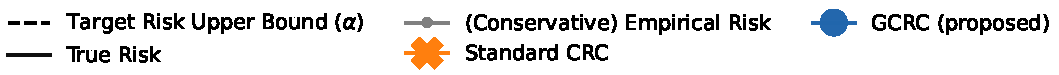
\includegraphics[width=\textwidth]{figures/legend1_crc_counterexample.pdf}}\\
    \begin{subfigure}{0.49\textwidth}
        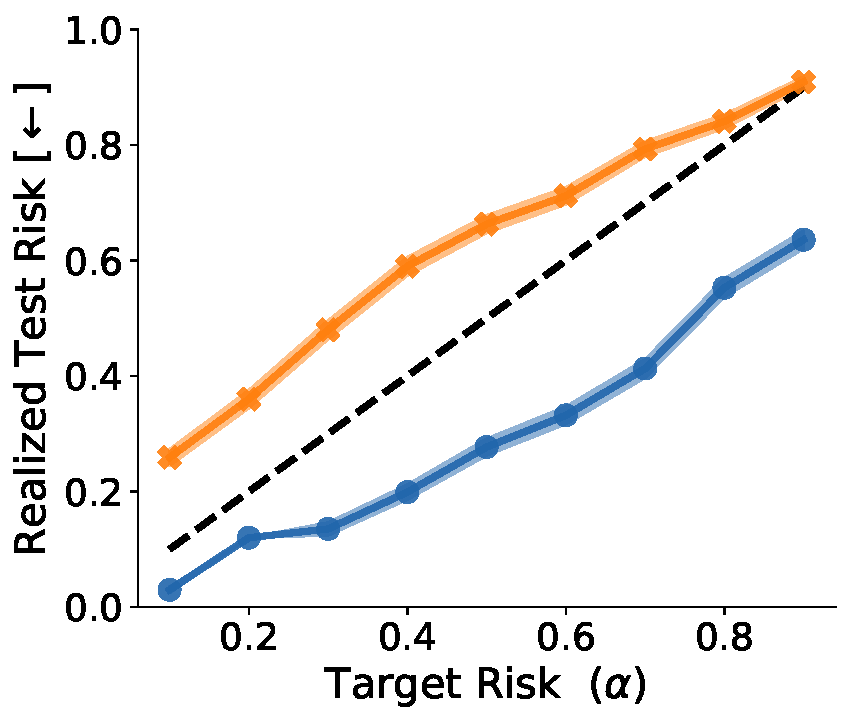
\includegraphics[width=\textwidth]{figures/counterexample_piecewise_loss_more_difficultLoss.pdf}
    \end{subfigure}
    \hfill
    \begin{subfigure}{0.49\textwidth}
        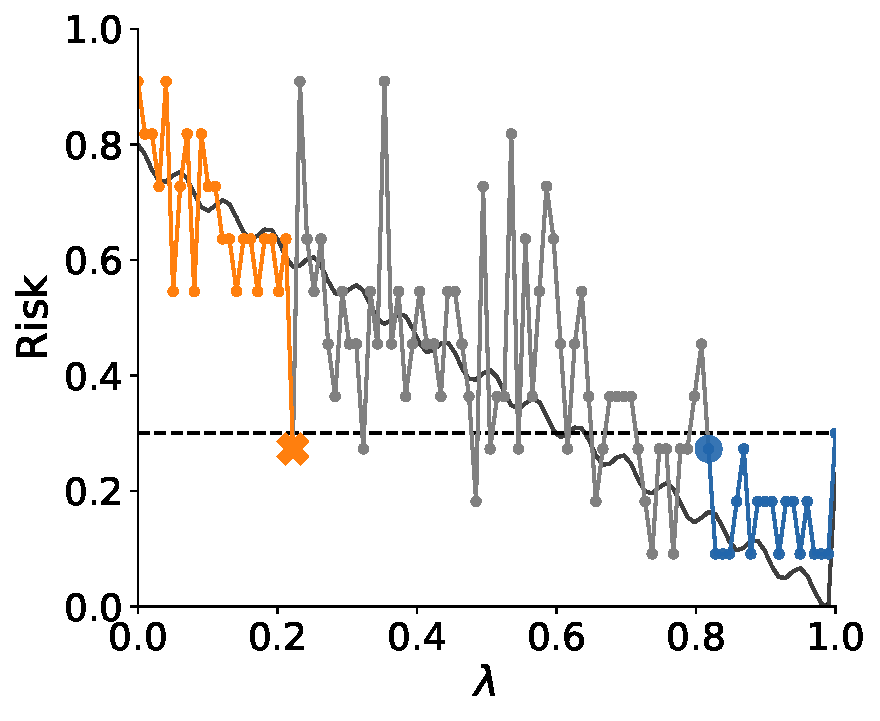
\includegraphics[width=\textwidth]{figures/empirical_risk_trajectory.pdf}
    \end{subfigure}
\end{subfigure}
\caption{Empirical comparison of standard CRC \citep{angelopoulos2022conformal} (orange) and the proposed generalized CRC (blue) on synthetic non-monotonic losses. gCRC achieves risk control across various target risk levels while CRC does not \textbf{(left)}. On an example empirical risk trajectory for these experiments, CRC underestimates the risk while gCRC maintains risk control by searching from safe to aggressive hyperparameter values \textbf{(right)}.}
\label{fig:CRC_counterexample}
\end{figure}

\textbf{Conformal methods:}
\citet{stanton2023bayesian} drew motivation from \citet{fannjiang2022conformal}, who first formalized the phenomenon of \textit{feedback covariate shift} to generalize conformal prediction to the setting of a single round of model-based optimization, building on techniques introduced by \citet{tibshirani2019conformal}.
\citet{prinster2024conformal} further extended these techniques to generalize conformal prediction for any data distribution, including showing coverage guarantees for the multi-round model-based optimization setting.

However, the techniques used throughout this line of work do not enable one to prescribe a data distribution (e.g., select a policy) that guarantees coverage.
That is, these methods can provide prediction sets with coverage guarantees for actions generated by any \textit{fixed} policy (a ``descriptive'' use of conformal techniques), but using those prediction sets to then \textit{select} a policy (a ``prescriptive'' use) introduces further, unaccounted-for dependence between the observed data and test policy that nullifies coverage guarantees.

To enable this prescriptive use case, we build upon techniques from conformal risk control (CRC) \cite{angelopoulos2022conformal}, a general framework for selecting a hyperparameter with finite-sample guarantees for any monotonic loss, of which conformal prediction can be cast as a special case.
When the loss of interest is non-monotonic, \citet{angelopoulos2022conformal} also showed that deploying the procedure on a monotonic relaxation of the losses provides asymptotic guarantees of control.
However, they left the problem of finite-sample guarantees for non-monotonic losses open.
In the next section, we develop a variant of CRC that drops the monotonicity requirement, and instead relies on smoothness of the losses and a form of stability of the calibration procedure to control the risk on the test point.
Finally, we apply techniques from \citet{prinster2024conformal} to prove finite-sample guarantees for our procedure in the multi-round model-based optimization setting.
See Appendix \ref{app:extended_related_work} for an extended discussion of related work.

\begin{figure*}[t]
    \centering
    \subfloat[$\beta \ll 1$]{
        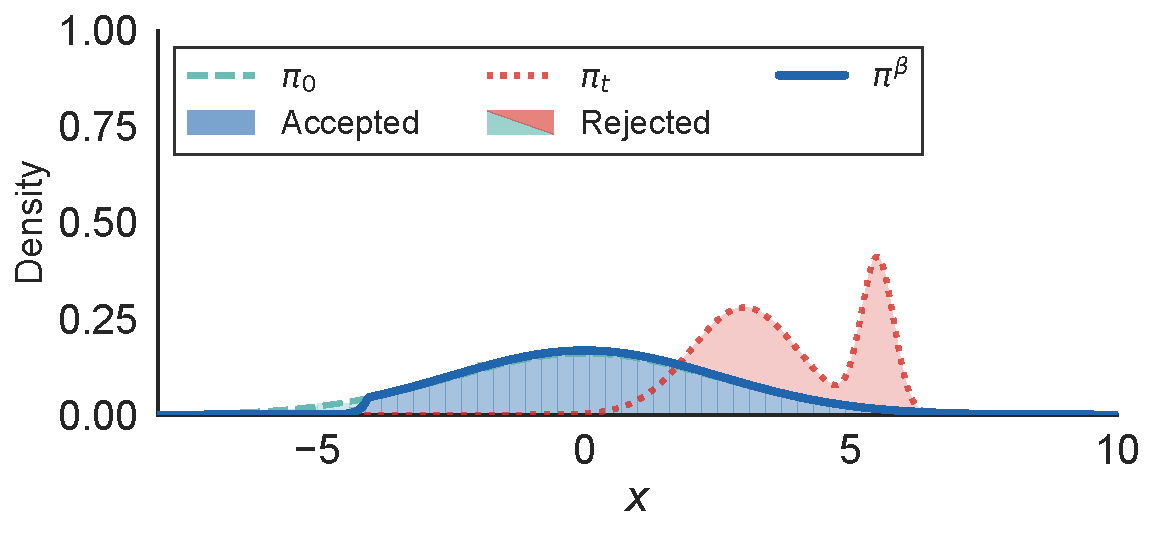
\includegraphics[width=0.33\textwidth]{figures/ar_beta_near_zero.pdf}
        \label{fig:ar_beta_near_zero}
    }
    \subfloat[$\beta = 1$]{
        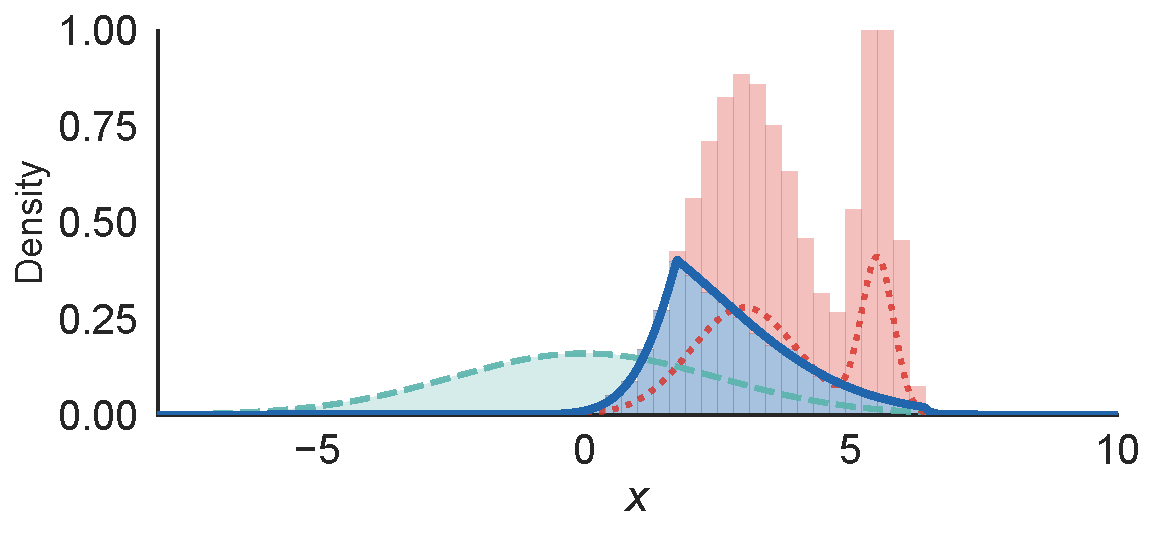
\includegraphics[width=0.33\textwidth]{figures/ar_beta_one.pdf}
        \label{fig:ar_beta_one}
    }
    \subfloat[$\beta \gg 1$]{
        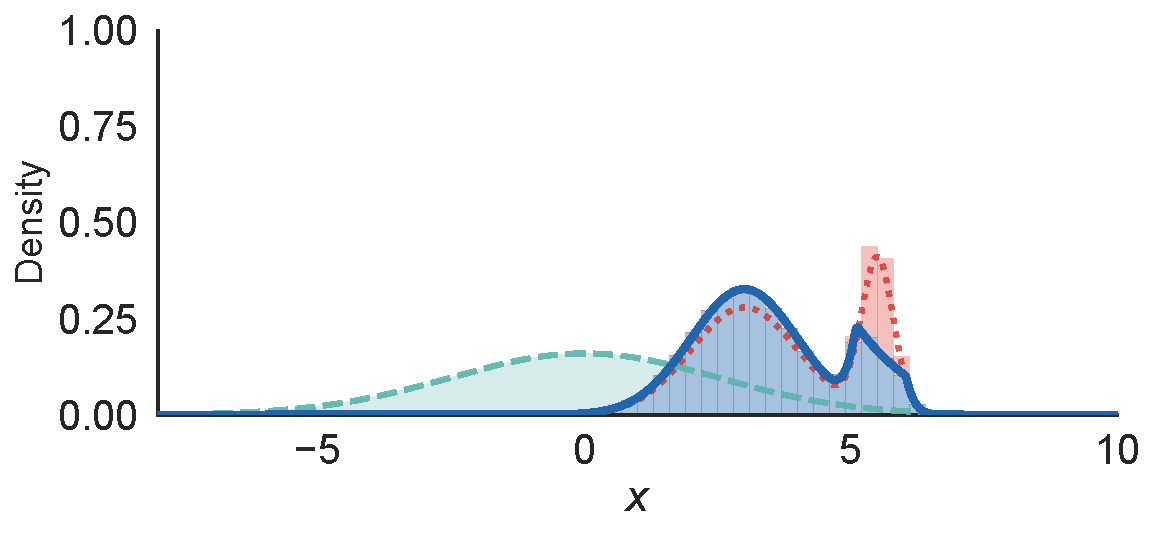
\includegraphics[width=0.33\textwidth]{figures/ar_beta_large.pdf}
        \label{fig:ar_beta_large}
    }
    \caption{Rejection sampling for policy interpolation at three $\beta$ values. 
    As $\beta$ increases from near-zero to large values, the constrained policy $\pi_t^{(\beta)}$
    interpolates from the safe policy $\pi_0$ to the optimized policy $\pi_t$. 
    Blue histogram bars show accepted samples matching $\pi_t^{(\beta)}$, while teal/red bars show
    rejected samples from the proposal distribution. (a) Small $\beta$ nearly recovers the safe policy (b) Intermediate $\beta$ shows intermediate interpolation with frequent rejections. (c) Large $\beta$ approaches the optimized policy with minimal rejection.}
    \label{fig:interpolating_distributions}
\end{figure*}


Concurrently, \citet{angelopoulos2026conformal} also present CRC guarantees for non-monotonic losses, but for parameterized losses, rather than the policy-control setting we introduce here where the control parameter tunes the policy instead of the loss. 
Even in the comparable setting of parameterized losses, however, the contributions are distinct, with neither subsuming the other: Relative to the univariate method in \citet{angelopoulos2026conformal}, our method (Section \ref{subsec:finite_sample_guarantees_crc_non_monotone}) will always be at least as conservative \textit{a priori} (e.g., as in Figure \ref{fig:CRC_counterexample}, right); consequently, whereas that paper's analogous guarantee relies on leave-one-out stability, our results use replace-one stability, which is generally a more relaxed assumption \citep{bousquet2002stability, shalev2010learnability}.
